\documentclass{article}

\newif\ifanswers
\answerstrue % comment out to hide answers

\usepackage{fancyhdr} % Required for custom headers
\usepackage{lastpage} % Required to determine the last page for the footer
\usepackage{extramarks} % Required for headers and footers
\usepackage[usenames,dvipsnames]{color} % Required for custom colors
\usepackage{graphicx} % Required to insert images
\usepackage{listings} % Required for insertion of code
\usepackage{courier} % Required for the courier font
\usepackage{lipsum} % Used for inserting dummy 'Lorem ipsum' text into the template
\usepackage{enumerate}
\usepackage{enumitem}
\usepackage{booktabs}
\usepackage{amsmath, amsthm, amssymb}
\usepackage{caption}
\usepackage{subcaption}
\captionsetup[table]{skip=4pt}
\usepackage{framed}
\usepackage{bm}
\usepackage[most]{tcolorbox}
\usepackage[colorlinks]{hyperref}


% guillaume edits
\usepackage{xcolor}
\graphicspath{{img/}} % set of paths to search for images
\usepackage{amsmath}
\usepackage{amsfonts}
\usepackage{amssymb}

\newenvironment{myitemize}
{ \begin{itemize}
		\setlength{\itemsep}{0pt}
		\setlength{\parskip}{0pt}
		\setlength{\parsep}{0pt}     }
	{ \end{itemize}                  } 
% end guillaume edits

\usepackage{biblatex} % bibliography
\addbibresource{papers.bib}

\usepackage{tikz}
\usetikzlibrary{positioning,patterns,fit}

\newcommand{\ifans}[1]{\ifanswers \color{red} \textbf{Solution: } #1 \color{black}}

% Margins
\topmargin=-0.45in
\evensidemargin=0in
\oddsidemargin=0in
\textwidth=6.5in
\textheight=9.0in
\headsep=0.25in

\linespread{1.1} % Line spacing

% Set up the header and footer
\pagestyle{fancy}
\rhead{\hmwkAuthorName} % Top left header
\lhead{\hmwkClass: \hmwkTitle} % Top center head
\lfoot{\lastxmark} % Bottom left footer
\cfoot{} % Bottom center footer
\rfoot{Page\ \thepage\ of\ \protect\pageref{LastPage}} % Bottom right footer
\renewcommand\headrulewidth{0.4pt} % Size of the header rule
\renewcommand\footrulewidth{0.4pt} % Size of the footer rule

\setlength\parindent{0pt} % Removes all indentation from paragraphs

%----------------------------------------------------------------------------------------
%	CODE INCLUSION CONFIGURATION
%----------------------------------------------------------------------------------------

\definecolor{MyDarkGreen}{rgb}{0.0,0.4,0.0} % This is the color used for comments
\lstloadlanguages{Python} % Load Perl syntax for listings, for a list of other languages supported see: ftp://ftp.tex.ac.uk/tex-archive/macros/latex/contrib/listings/listings.pdf
\lstset{language=Python, % Use Perl in this example
        frame=single, % Single frame around code
        basicstyle=\footnotesize\ttfamily, % Use small true type font
        keywordstyle=[1]\color{Blue}\bf, % Perl functions bold and blue
        keywordstyle=[2]\color{Purple}, % Perl function arguments purple
        keywordstyle=[3]\color{Blue}\underbar, % Custom functions underlined and blue
        identifierstyle=, % Nothing special about identifiers
        commentstyle=\usefont{T1}{pcr}{m}{sl}\color{MyDarkGreen}\small, % Comments small dark green courier font
        stringstyle=\color{Purple}, % Strings are purple
        showstringspaces=false, % Don't put marks in string spaces
        tabsize=5, % 5 spaces per tab
        %
        % Put standard Perl functions not included in the default language here
        morekeywords={rand},
        %
        % Put Perl function parameters here
        morekeywords=[2]{on, off, interp},
        %
        % Put user defined functions here
        morekeywords=[3]{test},
       	%
        morecomment=[l][\color{Blue}]{...}, % Line continuation (...) like blue comment
        numbers=left, % Line numbers on left
        firstnumber=1, % Line numbers start with line 1
        numberstyle=\tiny\color{Blue}, % Line numbers are blue and small
        stepnumber=5 % Line numbers go in steps of 5
}

% Creates a new command to include a perl script, the first parameter is the filename of the script (without .pl), the second parameter is the caption
\newcommand{\perlscript}[2]{
\begin{itemize}
\item[]\lstinputlisting[caption=#2,label=#1]{#1.pl}
\end{itemize}
}

%----------------------------------------------------------------------------------------
%	NAME AND CLASS SECTION
%----------------------------------------------------------------------------------------

\newcommand{\hmwkTitle}{Assignment \#3} % Assignment title
\newcommand{\hmwkClass}{CS\ 234} % Course/class
\newcommand{\hmwkAuthorName}{} % Your name

%----------------------------------------------------------------------------------------
%	TITLE PAGE
%----------------------------------------------------------------------------------------

\title{
\vspace{-1in}
\textmd{\textbf{\hmwkClass:\ \hmwkTitle\\
Winter 2019}}}
\date{} % Insert date here if you want it to appear below your name

\begin{document}

\maketitle
\vspace{-.5in}
\begin{framed}
\textbf{Due date: 2/27 11:59 PM PST}
\\[1em]
 We encourage students to discuss in groups for assignments. We ask
 that you abide by the university Honor Code and that of the Computer Science    department. If you have discussed the problems with others,
 please include a statement saying who you discussed problems with. Failure to   follow these instructions
 will be reported to the Office of Community Standards. We reserve the right to  run a fraud-detection software on your code. Please refer to the \href{http://web.  stanford.edu/class/cs234/index.html}{course website}, Academic Collaboration and Misconduct section for details about collaboration policy.
\\[1em]
Please review any additional instructions posted on the \href{http://cs234.stanford.edu/assignment3/index.html}{assignment page}. When you are ready to submit,
follow the instructions on the course website.
\end{framed}


\section{Policy Gradient Methods (50 pts coding + 15 pts writeup)}
The goal of this problem is to experiment with policy gradient and its variants, including variance reduction methods. Your goals will be to set up policy gradient for both continuous and discrete environments, and implement a neural network baseline for variance reduction. The framework for the vanilla policy gradient algorithm is setup in the starter code \texttt{pg.py}, and everything that you need to implement is in this file. The file has detailed instructions for each implementation task, but an overview of key steps in the algorithm is provided here. For this assignment you need to have \href{http://www.mujoco.org/index.html}{MuJoCo} installed, please follow the \href{https://drive.google.com/file/d/1PriAh0D3QSp2-5jLed-UohX9qH8j51zj/view}{installation guide}.

\subsection*{REINFORCE}
Recall the vanilla policy-gradient theorem,
\[ \nabla_\theta J(\theta) = \mathbb E_{\pi_\theta} \left[ \nabla_\theta \log\pi_\theta(a|s) Q^{\pi_\theta} (s,a) \right] \]
REINFORCE is a monte-carlo policy gradient algorithm, so we will be using the sampled returns $G_t$ as unbiased estimates of $Q^{\pi_\theta}(s,a)$. 
%So the gradient update becomes:
%\[ \nabla_\theta J(\theta) = \mathbb E_{\pi_\theta} \left[ \nabla_\theta \pi_\theta(s, a) G_t(s,a) \right] \]
Then the gradient update can be expressed as maximizing the following objective function:
\[ J(\theta) = \frac{1}{|D|} \sum_{\tau \in D} \sum_{t=1}^T \log(\pi_\theta(a_t|s_t)) G_t \]
where $D$ is the set of all trajectories collected by policy $\pi_\theta$, and $\tau=(s_0, a_0, r_0,s_1...,s_T)$ is a trajectory.

\subsection*{Baseline}
One difficulty of training with the REINFORCE algorithm is that the monte-carlo estimated return $G_t$ can have high variance. To reduce variance, we subtract a baseline $b_{\phi}(s)$ from the estimated returns when computing the policy gradient. A good baseline is the state value function parametrized by $\phi$, $b_{\phi}(s) = V^{\pi_\theta}(s)$, which requires a training update to $\phi$ to minimize the following mean-squared error loss:
\[ \mathcal{L}_{MSE}(\phi) = \frac{1}{|D|} \sum_{\tau \in D} \sum_{t=1}^T (b_{\phi}(s_t) - G_t)^2\]
\subsection*{Advantage Normalization}

After subtracting the baseline, we get the following new objective function:

\[ J(\theta) = \frac{1}{|D|} \sum_{\tau \in D} \sum_{t=1}^T \log(\pi_\theta(a_t|s_t)) \hat{A}_t \]

where

\[\hat{A}_t=G_t - b_{\phi}(s_t)\]

A second variance reduction technique is to normalize the computed advantages, $\hat{A}_t$, so that they have mean $0$ and standard deviation $1$. From a theoretical perspective, we can consider centering the advantages to be simply adjusting the advantages by a constant baseline, which does not change the policy gradient. Likewise, rescaling the advantages effectively changes the learning rate by a factor of $1/\sigma$, where $\sigma$ is the standard deviation of the empirical advantages.

\subsection{Coding Questions (50 pts)}
The functions that you need to implement in \texttt{pg.py} are enumerated here. Detailed instructions for each function can be found in the comments in \texttt{pg.py}. We strongly encourage you to look at \texttt{pg.py} and understand the code structure first.
\begin{itemize}
\item\texttt{build\_mlp}
\item\texttt{add\_placeholders\_op}
\item\texttt{build\_policy\_network\_op}
\item\texttt{add\_loss\_op}
\item\texttt{add\_optimizer\_op}
\item\texttt{add\_baseline\_op}
\item\texttt{get\_returns}
\item\texttt{calculate\_advantage}
\item\texttt{update\_baseline}
\end{itemize} 
\subsection{Writeup Questions (15 pts)}
\begin{enumerate}
\item[(a) (4 pts)] (CartPole-v0)
Test your implementation on the CartPole-v0 environment by running
\begin{tcolorbox}
\begin{verbatim}
python pg.py --env_name cartpole --baseline
\end{verbatim}
\end{tcolorbox}
With the given configuration file \texttt{config.py}, the average reward should reach $200$ within $100$ iterations. \emph{NOTE: training may repeatedly converge to 200 and diverge. Your plot does not have to reach 200 and stay there. We only require that you achieve a perfect score of 200 sometime during training.} 

Include in your writeup the tensorboard plot for the average reward. Start tensorboard with:
\begin{tcolorbox}
\begin{verbatim}
tensorboard --logdir=results
\end{verbatim}
\end{tcolorbox}
and then navigate to the link it gives you. Click on the ``SCALARS'' tab to view the average reward graph.

Now, test your implementation on the CartPole-v0 environment without baseline by running
\begin{tcolorbox}
\begin{verbatim}
python pg.py --env_name cartpole --no-baseline
\end{verbatim}
\end{tcolorbox}
Include the tensorboard plot for the average reward. Do you notice any difference? Explain.

\item[(b) (4 pts)](InvertedPendulum-v1)
Test your implementation on the InvertedPendulum-v1 environment by running
\begin{tcolorbox}
\begin{verbatim}
python pg.py --env_name pendulum --baseline
\end{verbatim}
\end{tcolorbox}

With the given configuration file \texttt{config.py}, the average reward should reach $1000$ within $100$ iterations. \emph{NOTE: Again, we only require that you reach 1000 sometime during training.} 

Include the tensorboard plot for the average reward in your writeup.

Now, test your implementation on the InvertedPendulum-v1 environment without baseline by running
\begin{tcolorbox}
\begin{verbatim}
python pg.py --env_name pendulum --no-baseline
\end{verbatim}
\end{tcolorbox}
Include the tensorboard plot for the average reward. Do you notice any difference? Explain.

\item[(c) (7 pts)](HalfCheetah-v1)
Test your implementation on the HalfCheetah-v1 environment with $\gamma = 0.9$ by running
\begin{tcolorbox}
\begin{verbatim}
python pg.py --env_name cheetah --baseline
\end{verbatim}
\end{tcolorbox}

With the given configuration file \texttt{config.py}, the average reward should reach $200$ within $100$ iterations. \emph{NOTE: There is some variance in training. You can run multiple times and report the best results or average. We have provided our results (average reward) averaged over 6 different random seed in figure \ref{fig:half}} Include the tensorboard plot for the average reward in your writeup.

Now, test your implementation on the HalfCheetah-v1 environment without baseline by running
\begin{tcolorbox}
\begin{verbatim}
python pg.py --env_name cheetah --no-baseline
\end{verbatim}
\end{tcolorbox}
Include the tensorboard plot for the average reward. Do you notice any difference? Explain.
\end{enumerate}
% We have provided our results for HalfCheetah-v1's average reward for your reference. Note that this result is averaged over 6 different random seeds.
\begin{figure}[h]
    \centering
    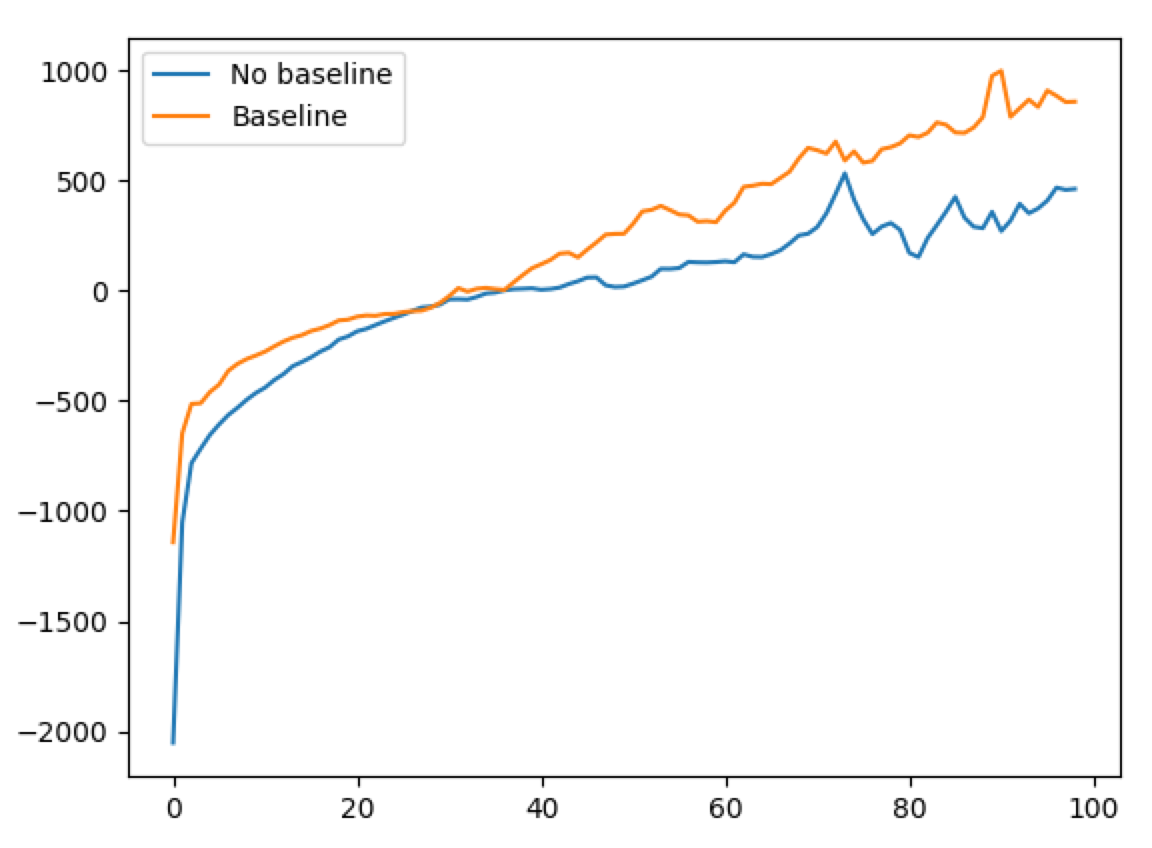
\includegraphics[width=0.25\linewidth]{halfcheetah.png}
    \caption{Half Cheetah, averaged over 6 runs}
    \label{fig:half}
\end{figure}
 
 \newpage

\section{Best Arm Identification in Multiarmed Bandit (35pts)}
In this problem we focus on the Bandit setting with rewards bounded in $[0,1]$. A Bandit problem instance is defined as an MDP with just one state and action set $\mathcal A$. Since there is only one state, a ``policy'' consists of the choice of a single action: there are exactly $A = |\mathcal A|$ different deterministic policies. Your goal is to design a simple algorithm to identify a near-optimal arm with high probability.

Imagine we have $n$ samples of a random variable $x$, $\{x_1, \dots, x_n\}$. We recall Hoeffding's inequality below, where $\overline x$ is the expected value of a random variable $x$, $\widehat x= \frac{1}{n} \sum_{i=1}^n x_i$ is the sample mean (under the assumption that the random variables are in the interval [0,1]), $n$ is the number of samples  and $\delta >0$ is a scalar:

\begin{align*}
\Pr\Bigg(|\widehat x - \overline x | > \sqrt{\frac{\log(2/\delta)}{2n}}	\Bigg) < \delta.
\end{align*}

Assuming that the rewards are bounded in $[0,1]$,
we propose this simple strategy: allocate an identical number of samples $n_1 = n_2=...=n_{A} = n_{des}$ to every action, compute the average reward (empirical payout) of each arm $\widehat r_{a_1}, \dots, \widehat r_{a_A}$ and return the action with the highest empirical payout $\arg\max_a \widehat r_{a}$. The purpose of this exercise is to study the number of samples required to output an arm that is at least $\epsilon$-optimal with high probability.
Intuitively, as $n_{des}$ increases the empirical payout $\widehat r_a$ converges to its expected value $\overline r_a$ for every action $a$, and so choosing the arm with the highest empirical payout $\widehat r_a$ corresponds to approximately choosing the arm with the highest expected payout $\overline r_a$.

\begin{enumerate}
\item[(a) (15 pts)] We start by defining a \emph{good event}. Under this \emph{good event}, the empirical payout of each arm is not too far from its expected value. Starting from Hoeffding inequality with $n_{des}$ samples allocated to every action show that:

\begin{align*}
\Pr\Bigg(\exists a \in \mathcal A \quad s.t. \quad |\widehat r_a - \overline r_a | > \sqrt{\frac{\log(2/\delta)}{2n_{des}}}	\Bigg) < A\delta.
\end{align*}

In other words, the \emph{bad event} is that at least one arm has an empirical mean that differs significantly from its expected value and this has probability at most $A\delta$.

\item[(b) (20 pts)] After pulling each arm (action) $n_{des}$ times our algorithm returns the arm with the highest empirical payout:
\begin{equation*}
a^\dagger = argmax_{a} \widehat r_a	
\end{equation*}
Notice that $a^\dagger$ is a random variable.
 Define ${a^\star}$ as the optimal arm (that yields the highest average reward ${a^\star} = argmax_a \overline r_{a}$). Suppose that we want our algorithm to return at least an $\epsilon$ optimal arm with probability $1-\delta'$, as follows:

\begin{equation*}
	\Pr \Bigg(\overline r_{a^\dagger} \geq  \overline r_{a^\star} - \epsilon \Bigg) \geq 1-\delta'.
\end{equation*}
How many samples are needed to ensure this? Express your result as a function of the number of actions $A$, the required precision $\epsilon$ and the failure probability $\delta'$.
\end{enumerate}

\printbibliography



\end{document}
